\section[Combinatorial mutations of the PM polygon are realized\\ by extended deformations]{Combinatorial mutations of the PM polygon are realized\\ by extended deformations}
\label{mutation_vs_deformation}

Throughout this section, we still keep the notation of Sections~\ref{sec_def_deform} and~\ref{sec_def_exdeform} unless otherwise stated.
In this section, we show that the combinatorial mutation of the PM polygon of a consistent dimer model coincides with the PM polygon of the deformed dimer model (see Theorem~\ref{mutation=deformation}).
First, we observe the relationship between the deformation data (see Definition~\ref{def_deformation_data}) and the mutation data (see Definition~\ref{def_mutation_data}).

\begin{setting}
\label{mutation_deformation_setting}
Let $\Gamma$ be a reduced consistent dimer model, and $\Delta_\Gamma$ be the PM polygon of $\Gamma$.
We take a type I zigzag path $z$ of $\Gamma$ with $v\coloneqq [z]\in\ZZ^2$. Then, by Proposition~\ref{zigzag_sidepolygon}
there is an edge $E$ of $\Delta_\Gamma$ whose outer normal vector is $v$.
Since $\Delta_\Gamma$ is determined up to translation, there is ambiguity concerning the position of the origin.
Thus, we fix the origin ${\bf 0}$ for $\Delta_\Gamma$ so that ${\bf 0}\in\Delta_\Gamma$.
Let $w\coloneqq -v$, and consider
\begin{gather*}
h_{\max}= h_{\max}(\Delta_\Gamma,w)\coloneqq{\max}\{\langle w,u\rangle \,|\, u\in \Delta_\Gamma\},
\\
h_{\min}= h_{\min}(\Delta_\Gamma,w)\coloneqq{\min}\{\langle w,u\rangle \,|\, u\in \Delta_\Gamma\}.
\end{gather*}
Now, we let $r\coloneqq-h_{\min}$ and assume that $r\le\big|\calZ_v^\rmI(\Gamma)\big|$.
Since the length of the line segments of~$E$ is~$|E\cap N|-1$ and this is equal to $|\calZ_v(\Gamma)|$ by Proposition~\ref{zigzag_sidepolygon}, we have
\begin{displaymath}
-h_{\min}=r\le|\calZ_v^\rmI(\Gamma)|\le|\calZ_v(\Gamma)|=|E\cap N|-1.
\end{displaymath}
Thus $\Delta_\Gamma$ admits the combinatorial mutation with respect to~$w$ (see Remark~\ref{rem_def_mutation}).
Let $\ell(z)\coloneqq2n$. Then, by Lemma~\ref{zigzag_lem1} we have
\begin{align*}
n=\ell(z)/2&=|\sfP\cap z|+\langle h(\sfP,\sfP_i),w\rangle =|\sfP\cap z|+\langle h(\sfP,\sfP_0)-h(\sfP_i,\sfP_0),w\rangle\\
&=|\sfP\cap z|+\langle h(\sfP,\sfP_0),w\rangle-\langle h(\sfP_i,\sfP_0),w\rangle,
\end{align*}
where $\sfP$ is a perfect matching on $\Gamma$, $\sfP_0$ is the reference perfect matching, and $\sfP_i\in\PM_{\max}(z)$.
Since $h(\sfP_i,\sfP_0)$ is a lattice point on $E$ by Lemma~\ref{number_zigzag_corner}, we have $\langle h(\sfP_i,\sfP_0),w\rangle=h_{\min}$.
If $\sfP\in\PM_{\min}(z)$, then $|\sfP\cap z|=0$ by Lemma~\ref{lem_existence_pm}, and this means that $\langle h(\sfP,\sfP_0),w\rangle=h_{\max}$.
Thus, we have $n=h_{\max}-h_{\min}=\width(\Delta_\Gamma,w)$.


We show how the correspondence between mutation data and deformation data in Table~\ref{mutation_deformation_data}.

\begin{table}[h!]\centering
\begin{tabular}{|c|c|}
\hline
Mutation data&Deformation data \\ \hline
$w$&$-v$ \\ \hline
$h_{\min}$&$-r$\\ \hline
$h_{\max}$&$h$ \\ \hline
$\width(\Delta_\Gamma,w)$&$n$ \\ \hline
\end{tabular}

\caption{Relationships between the mutation data and the deformation data.}\label{mutation_deformation_data}
\end{table}

Using the integers $r$, $h$, we take type I zigzag paths $z_1,\dots,z_r$ and the zig-deformation (resp.\ zag-deformation) parameter~$\calX$ (resp.~$\calY$) with respect to $z_1,\dots,z_r$ as in Setting~\ref{def_deformation_exdata}.
We then have the deformed consistent dimer models $\nu^\zig_\calX(\Gamma)=\nu^\zig_\calX(\Gamma, \{z_1,\dots,z_r\})$
and $\nu^\zag_\calY(\Gamma)=\nu^\zag_\calY(\Gamma, \{z_1,\dots,z_r\})$.

We determine the origin of the PM polygons $\Delta_{\nu^\zig_\calX(\Gamma)}$ and $\Delta_{\nu^\zag_\calY(\Gamma)}$ as follows.
First, there are zigzag paths $y_1^\prime,\dots,y_t^\prime$ on $\nu^\zig_\calX(\Gamma)$ whose slope respectively corresponds to the one of zigzag paths $y_1,\dots, y_t$ on $\Gamma$ by Proposition~\ref{zigzag_afterdeform1}.
Then, we put $\Delta_{\nu^\zig_\calX(\Gamma)}$ on $\Delta_\Gamma$ so that the edges corresponding to $y_1^\prime,\dots,y_t^\prime$ respectively coincide with the edges of $\Delta_\Gamma$ corresponding to $y_1,\dots,y_t$.
We determine the origin for $\Delta_{\nu^\zig_\calX(\Gamma)}$ so that it is in the same position as the origin for $\Delta_\Gamma$.
Considering the zigzag paths on $\nu^\zag_\calY(\Gamma)$ obtained from the zigzag paths $x_1,\dots,x_s$ on $\Gamma$,
we can also determine the origin for $\Delta_{\nu^\zag_\calY(\Gamma)}$.
\end{setting}

\begin{Remark}
\label{rem_typeI_isoradial}
In Setting~\ref{mutation_deformation_setting}, we assumed that $r\le|\calZ_v^\rmI(\Gamma)|$ for defining the deformation data.
As we mentioned in Remark~\ref{rem_typeI_to_typeII}, even if the number of type I zigzag paths is insufficient,
we can sometimes change a type II zigzag path into a type I zigzag path without changing the PM polygon by using mutations of dimer models (see Appendix~\ref{app_mutationdimer}).
Moreover, it is known that for a given lattice polygon $P$ there exists an isoradial dimer model giving $P$ as the PM polygon by~\cite{Gul}, in which case all zigzag paths are type I (see Definition~\ref{def_isoradial}), and hence $\big|\calZ_v^\rmI(\Gamma)\big|=|\calZ_v(\Gamma)|$.
Thus, if $-h_{\min}\le|E\cap N|-1$ we can find a certain isoradial dimer model $\Gamma$ satisfying $-h_{\min}=r\le|\calZ_v^{\rmI}(\Gamma)|=|E\cap N|-1$.
\end{Remark}

For any edge $E$ of $\Delta_\Gamma$ as in Setting~\ref{mutation_deformation_setting}, we take a primitive lattice element $u_E\in N$ such that $\langle w,u_E\rangle=0$.
Here, there are two choices of~$u_E$ and we fix~$u_E$ as follows.
We recall the primitive lattice element $h(\sfP^\prime_z,\sfP_z)$ given in Settings~\ref{setting_PMs_z}, which satisfies $\langle[z],h(\sfP^\prime_z,\sfP_z)\rangle=0$.
We let $u_E\coloneqq h(\sfP^\prime_z,\sfP_z)$, and hence $\langle w,u_E\rangle=\langle-[z],u_E\rangle=0$.
We set the line segment $F$ as $F\coloneqq \operatorname{conv}\{{\bf 0},u_E\}$.
Using this with Setting~\ref{mutation_deformation_setting} (and also Table~\ref{mutation_deformation_data}),
our main theorem can be stated as follows.

\begin{Theorem}\label{mutation=deformation}
Let $\Gamma$ be a reduced consistent dimer model with ${\bf 0}\in\Delta_\Gamma$.
Then, we have
\begin{gather*}
\mutation_{w}(\Delta_\Gamma,F)=\Delta_{\nu^\zig_\calX(\Gamma,\{z_1,\dots,z_r\})},\\
\mutation_{w}(\Delta_\Gamma,-F)=\Delta_{\nu^\zag_\calY(\Gamma,\{z_1,\dots,z_r\})}.
\end{gather*}
\end{Theorem}

\begin{proof}We will prove the first equation. The other one follows from a similar argument.

First, we show that
\begin{displaymath}
\varphi(\Delta_\Gamma^*)=\Delta_{\nu^\zig_\calX(\Gamma,\{z_1,\dots,z_r\})}^*,
\end{displaymath}
where $\varphi=\varphi_{w,F}$ is the map given in (\ref{mutation_M}).

Let $E_1\coloneqq E, E_2,\dots,E_m$ be the edges of $\Delta_\Gamma$ ordered cyclically in the anti-clockwise direction.
As we mentioned in Setting~\ref{mutation_deformation_setting}, we suppose that ${\bf 0}\in\Delta_\Gamma$.
Let $w_1\coloneqq w,w_2, \dots, w_m$ be inner normal vectors corresponding to $E_1,\dots,E_m$, respectively (see Figure~\ref{PMpolygon_normalvec}).
Also, we let $v_i=-w_i$ for $i=1,\dots,r$, which are the outer normal vectors corresponding to $E_i$.
We then consider $u\in\Delta_\Gamma$ such that $\langle w_1,u\rangle=h_{\max}(\Delta_\Gamma,w_1)=h$; that is, we consider $w_{h_{\max}}(\Delta_\Gamma)$, which is either a~vertex or an edge of $\Delta_\Gamma$.
If $w_{h_{\max}}(\Delta_\Gamma)$ is an edge, we easily see that it is parallel to $E$, in which case we may write $E_a\coloneqq w_{h_{\max}}(\Delta_\Gamma)$ for some $1<a<m$.
If $w_{h_{\max}}(\Delta_\Gamma)$ is a vertex, we set the edges intersecting at $w_{h_{\max}}(\Delta_\Gamma)$ as $E_{a-1}$, $E_{a+1}$ and set $E_a=\varnothing$ where $1<a<m$.
Recall that by Proposition~\ref{zigzag_sidepolygon}, for each $E_i\neq\varnothing$ there exist zigzag paths on $\Gamma$ such that the slopes coincide with $v_i$,
and the set of such zigzag paths is denoted by $\calZ_{v_i}=\calZ_{v_i}(\Gamma)$.

\begin{figure}[h!]\centering
\scalebox{0.9}{
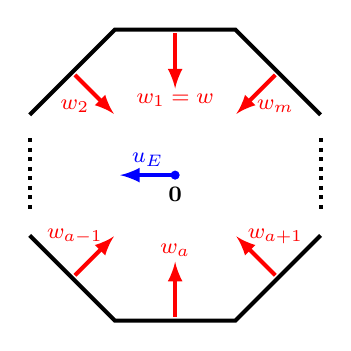
\begin{tikzpicture}[sarrow/.style={-latex, very thick}]
\foreach \name/\r in {0/2,1/2,2/2,3/2,4/2,5/2,6/2,7/2}{\coordinate (v\name) at (22.5+45*\name:\r cm);}
\draw [line width=0.05cm] (v0)--(v1)--(v2)--(v3); \draw [line width=0.05cm] (v4)--(v5)--(v6)--(v7);

\path (v3) ++(-90:0.3cm) coordinate (v3-); \path (v4) ++(90:0.3cm) coordinate (v4+);
\draw [line width=0.05cm, dotted] (v3-)--(v4+);
\path (v0) ++(-90:0.3cm) coordinate (v0-); \path (v7) ++(90:0.3cm) coordinate (v7+);
\draw [line width=0.05cm, dotted] (v0-)--(v7+);

\foreach \name in {1,2,3,5,6,7}{\coordinate (vec\name) at (45*\name:1.8 cm);}
\foreach \name in {1,2,3,5,6,7}{\draw[red, sarrow, line width=0.05cm] (vec\name)-- ++(180+45*\name:0.7cm);}

\path (vec1) ++(-90:0.4cm) node[red] {\footnotesize$w_m$};
\path (vec2) ++(-90:0.85cm) node[red] {\footnotesize$w_1=w$};
\path (vec3) ++(-90:0.4cm) node[red] {\footnotesize$w_2$};
\path (vec5) ++(90:0.5cm) node[red] {\footnotesize$w_{a-1}$};
\path (vec6) ++(90:0.85cm) node[red] {\footnotesize$w_a$};
\path (vec7) ++(90:0.5cm) node[red] {\footnotesize$w_{a+1}$};
\filldraw [blue] (0,0) circle [radius=0.05cm];
\draw[blue, sarrow, line width=0.05cm] (0,0)-- ++(180:0.7cm) node[inner sep=0.5pt, circle, midway, xshift=0cm, yshift=0.2cm, blue] {\footnotesize$u_E$};
\node at (0,-0.25) {\footnotesize${\bf 0}$};
\end{tikzpicture}
}
\caption{The PM polygon $\Delta_\Gamma$ and its inner normal vectors (the case where the origin is contained in the strict interior of $\Delta_\Gamma$).}
\label{PMpolygon_normalvec}
\end{figure}

First, we consider the edge $E_1$ and zigzag paths in $\calZ_{v_1}=\calZ_{(-w)}$.
By definition, we have $\langle -v_1,u_E\rangle=0$ and $\{z_1,\dots,z_r\}\subseteq\calZ_{(-w)}^\rmI\subseteq \calZ_{(-w)}$.
If $|\calZ_{(-w)}|>r$, then there exists a zigzag path in $\calZ_{(-w)}$ that is not in $\{z_1,\dots,z_r\}$.
If $E_a\neq\varnothing$, we have zigzag paths in $\calZ_{v_a}$.
Since $E_1$ and $E_a$ are parallel, $v_1$ and $v_a$ are linearly dependent, and hence $\langle v_a,u_E\rangle=0$.
Then, we see that zigzag paths in $\calZ_{v_a}$ do not intersect with any type I zigzag path $z$ satisfying $[z]=v_1$ in the universal cover (see Lemma~\ref{slope_linearly_independent}).

Next, we consider the edges $E_2,\dots,E_{a-1}$ of $\Delta_\Gamma$ and zigzag paths in $\calZ_1\coloneqq\calZ_{v_2}\cup\cdots\cup\calZ_{v_{a-1}}$.
We see that $v_i$ with $i=2,\dots,a-1$ satisfies $\langle -v_i,u_E\rangle<0$ by a choice of the edges $E_2,\dots,E_{a-1}$.
By the same argument as in the proof of Proposition~\ref{prop_nondegenerate}, we see that
the zigzag paths in $\calZ_1$ intersect with a type I zigzag path $z$ satisfying $[z]=v_1$ precisely once in the universal cover (see Lemma~\ref{slope_linearly_independent}); specifically, they intersect with $z$ in $\Zag(z)$.
Thus, we have $\calZ_1=\{x_1,\dots,x_s\}$, and for each $i=2,\dots ,a-1$ the vector $v_i$ satisfies $v_i=[x_j]$ for some $j=1,\dots,s$.

Next, we consider the edges $E_{a+1},\dots,E_m$ of $\Delta_\Gamma$ and zigzag paths in $\calZ_2\coloneqq\calZ_{v_{a+1}}\cup\cdots\allowbreak\cup\calZ_{v_m}$.
We see that~$v_i$ with $i=a+1,\dots,m$ satisfies $\langle -v_i,u_E\rangle>0$ by the choice of the edges $E_{a+1},\dots,E_m$.
By a similar argument as above, we see that the zigzag paths in $\calZ_2$ intersect with a type I zigzag path $z$ satisfying $[z]=v_1$ precisely once in the universal cover; specifically, they intersect with $z$ in $\Zig(z)$.
Thus, we have $\calZ_2=\{y_1,\dots,y_t\}$, and for each $i=a+1,\dots,m$ the vector $v_i$ satisfies $v_i=[y_k]$ for some $k=1,\dots,t$.

Collectively, we see that any zigzag path of $\Gamma$ takes one of the following forms:
\begin{itemize}\itemsep=0pt
\item $z_1,\dots,z_r$,
\item $z_1^\prime,\dots,z_{r^\prime}^\prime$ contained in $\calZ_{(-w)}{\setminus}\{z_1,\dots,z_r\}$ for $w=-v_1$ with $\langle w,u_E\rangle=0$ if $|\calZ_{(-w)}|>r$,
\item $z_1^{\prime\prime},\dots,z_{r^{\prime\prime}}^{\prime\prime}$ contained in $\calZ_w$ for $w=-v_1$ with $\langle w,u_E\rangle=0$ if $E_a\neq\varnothing$,
\item $x_j$ where $j=1,\dots,s$, in which case it satisfies $\langle-[x_j],u_E\rangle<0$,
\item $y_k$ where $k=1,\dots,t$, in which case it satisfies $\langle-[y_k],u_E\rangle>0$.
\end{itemize}
The slopes of these zigzag paths give the supporting hyperplanes of $\Delta_\Gamma$ by Proposition~\ref{zigzag_sidepolygon}. More precisely, if $\Delta_\Gamma$ contains the origin ${\bf 0}$ as an interior lattice point, then
\begin{displaymath}
H_{-[\zeta],\ge -k_\zeta}=\{u\in N_\RR\,|\,\langle-[\zeta],u\rangle\ge -k_\zeta\}
\end{displaymath}
is the supporting hyperplane of $\Delta_\Gamma$ for any zigzag path $\zeta$ of $\Gamma$ and a certain positive integer $k_\zeta$.
If the origin ${\bf 0}$ lies on the boundary of $\Delta_\Gamma$, $k_\zeta$ is replaced by $0$ for the zigzag paths corresponding to the edges that contain ${\bf 0}$.
By Proposition~\ref{prop_dual_polytope} and its proof, $\Delta_\Gamma^*$ can be written as $\Delta_\Gamma^*=Q+C$, where $Q$ is a polygon and $C$ is a polyhedral cone.
Since the set of the slopes of zigzag paths of $\Gamma$ coincides with $\{v_1,\dots,v_m\}$ if we identify the same slopes,
we see that the set $\{u_1,\dots,u_p,u_1^\prime,\dots,u_q^\prime\}$, which generates $Q$ and $C$ in the proof of Proposition~\ref{prop_dual_polytope},
is given by $\{w_1,\dots,w_m\}$ in our situation.
In what follows, we assume that ${\bf 0}$ is contained in the strict interior of $\Delta_\Gamma$, in which case $\Delta_\Gamma^*=Q$ and
$Q=\operatorname{conv}\big(\big\{\frac{1}{k_1}w_1,\dots,\frac{1}{k_m}w_m\big\}\big)$ for some positive integers $k_i$,
giving the supporting hyperplanes $H_{w_i,\ge-k_i}$ of $\Delta_\Gamma$ for $i=1,\dots,m$.
We remark that $\frac{1}{k_a}w_a$ appears in the above generating set if $E_a\neq\varnothing$.
Since $\langle w_i,u_E\rangle\ge0$ for $i=1,a, a+1,\dots, m$ and $\langle w_i,u_E\rangle<0$ for $i=2,\dots, a-1$,
we see that
\begin{gather}
\varphi(\Delta_\Gamma^*)=\operatorname{conv}\bigg(\bigg\{\frac{1}{k_1}w_1,\frac{1}{k_2}w_2^\prime,\dots,\frac{1}{k_{a-1}}w_{a-1}^\prime,
\frac{1}{k_a}w_a \ \text{(if $E_a\neq\varnothing$)}, \nonumber\\
\hphantom{\varphi(\Delta_\Gamma^*)=\operatorname{conv}\bigg(\bigg\{}{}
\frac{1}{k_{a+1}}w_{a+1}, \dots,\frac{1}{k_m}w_m\bigg\}\bigg),\label{generating_set_dual}
\end{gather}
where $w_i^\prime\coloneqq w_i-\langle w_i,u_E\rangle w$ for $i=2,\dots,a-1$.
We also note that when $E_a=\varnothing$, we can take the positive integer $k_a$ so that the line $\{u\in N_\RR\,|\,\langle v_1,u\rangle= -k_a\}$, which is parallel to $E_1$, passes through the vertex of $\Delta_\Gamma$ that is the intersection of $E_{a-1}$ and $E_{a+1}$.
By the choice of $k_a$, we have $\langle \frac{1}{k_a}v_1,u\rangle\ge -1$ for any $u\in \Delta_\Gamma$; thus $\frac{1}{k_a}v_1=\frac{1}{k_a}(-w_1)\in\Delta_\Gamma^*$ and hence $\frac{1}{k_a}v_1=\frac{1}{k_a}(-w_1)\in\varphi(\Delta_\Gamma^*)$.

We then consider the deformed dimer model $\nu^\zig_\calX(\Gamma)=\nu^\zig_\calX(\Gamma,\{z_1,\dots,z_r\})$.
By Observation~\ref{obs_deformed_part}, the lift of any zigzag path of the form $z_i^\prime$ or $z_i^{\prime\prime}$ on the universal cover is contained in some irrelevant part, and hence it does not change even if we apply the extended deformation.
Also, by Proposition~\ref{zigzag_afterdeform2}, we have the zigzag paths $x_1^\prime,\dots,x_s^\prime$ on $\nu^\zig_\calX(\Gamma)$ satisfying
\begin{displaymath}
-[x^{\prime}_j]=-[x_j]-\langle [x_j],h(\sfP_z^\prime,\sfP_z)\rangle[z]=w_i-\langle w_i,u_E\rangle w
\end{displaymath}
for $j=1,\dots,s$ and some $i=2,\dots,a-1$.
Furthermore, by Proposition~\ref{zigzag_afterdeform1}, we have the zigzag paths $y_1^\prime,\dots,y_t^\prime$ on $\nu^\zig_\calX(\Gamma)$ satisfying
\begin{displaymath}
-[y_k^\prime]=-[y_k]=w_i
\end{displaymath}
for $k=1,\dots,t$ and some $i=a+1,\dots,m$.
Thus, we see that the zigzag paths $x_j, y_k$ vary as they satisfy the condition (\ref{mutation_M}) when we apply the extended deformation $\nu^\zig_\calX$ to $\Gamma$.
In addition, we have the zigzag path of the form $z_{i,j}$ defined in (zig-3).
Thus, the zigzag paths on the consistent dimer model $\nu^\zig_\calX(\Gamma)$ are
\begin{gather*}
\{z_i^\prime\}_{1\le i\le r^\prime}\quad \text{(if $|\calZ_{(-w)}|>r$)},\qquad \{z_i^{\prime\prime}\}_{1\le i\le r^{\prime\prime}}\quad \text{(if $E_a\neq\varnothing$)},\\
\{x_j^\prime\}_{1\le j\le s},\qquad \{y_k^\prime\}_{1\le k\le t},\qquad \text{and} \qquad \{z_{i,j}\}_{\substack{1\le i\le r \\ 1\le j\le p_i}}.
\end{gather*}
By the description of their slopes and Proposition~\ref{zigzag_sidepolygon}, we see that the inner normal vectors of~$\Delta_{\nu^\zig_\calX(\Gamma)}$ are
\begin{displaymath}
\{w_1,w_2^\prime,\dots,w_{a-1}^\prime,w_a=-w_1, w_{a+1}, \dots,w_m\},
\end{displaymath}
and these vectors give the supporting hyperplanes of $\Delta_{\nu^\zig_\calX(\Gamma)}$ just like for $\Delta_\Gamma$.
Here, $w_1$ appears in the above set if $|\calZ_{(-w_1)}|=|\calZ_{v_1}|>r$,
but we always have $\frac{1}{k_1}w_1\in \Delta_{\nu^\zig_\calX(\Gamma)}^*$ by the same argument as we used for showing $\frac{1}{k_a}(-w_1)\in\Delta_\Gamma^*$ above, whereas $w_a$ certainly appears since $[z_{i,j}]=-[z_i]=-w_1=w_a$ (see Lemma~\ref{deform_vector}). Thus, we have
\begin{displaymath}
\Delta_{\nu^\zig_\calX(\Gamma)}^*=\operatorname{conv}\bigg(\bigg\{\frac{1}{k_1}w_1,\frac{1}{k_2}w_2^\prime,\dots,\frac{1}{k_{a-1}}w_{a-1}^\prime,
\frac{1}{k_a}w_a, \frac{1}{k_{a+1}}w_{a+1}, \dots,\frac{1}{k_m}w_m\bigg\}\bigg).
\end{displaymath}
By the description (\ref{generating_set_dual}) and the fact that $\frac{1}{k_1}w_1$ and $\frac{1}{k_a}w_a=\frac{1}{k_a}(-w_1)$ are contained in both $\varphi(\Delta_\Gamma^*)$ and $\Delta_{\nu^\zig_\calX(\Gamma)}^*$, we see that $\varphi(\Delta_\Gamma^*)=\Delta_{\nu^\zig_\calX(\Gamma)}^*$.

The case where the origin ${\bf 0}$ lies on the boundary of $\Delta_\Gamma$ can be proved by a similar argument if we consider the hyperplane $\{u\in N_\RR\,|\,\langle-[\zeta],u\rangle\ge 0\}$ instead of $\{u\in N_\RR\,|\,\langle-[\zeta],u\rangle\ge -k_\zeta\}$ for the zigzag paths corresponding to the edges that contain ${\bf 0}$, in which case $-[\zeta]$ will be a~generator of a polyhedral cone~$C$.

By Propositions~\ref{prop_dual_polytope}(ii) and \ref{prop_mutation_dual_polytope}, we conclude that
$\mutation_{w}(\Delta_\Gamma,F)=\Delta_{\nu^\zig_\calX(\Gamma)}$.
\end{proof}
